%% 2/18/2016
%%%%%%%%%%%%%%%%%%%%%%%%%%%%%%%%%%%%%%%%%%%%%%%%%%%%%%%%%%%%%%%%%%%%%%%%%%%%
% AGUJournalSample.tex: this sample file is for articles formatted with LaTeX
%
% This sample file includes commands and instructions
% given in the order necessary to produce a final output that will
% satisfy AGU requirements.
%
% PLEASE DO NOT USE YOUR OWN MACROS
% DO NOT USE \newcommand, \renewcommand, or \def.
%
% FOR FIGURES, DO NOT USE \psfrag or \subfigure.
% DO NOT USE \psfrag or \subFig. commands.
%
%%%%%%%%%%%%%%%%%%%%%%%%%%%%%%%%%%%%%%%%%%%%%%%%%%%%%%%%%%%%%%%%%%%%%%%%%%%%
%
% Step 1: Set the \documentclass
%
% There are two options for article format:
%
% 1) PLEASE USE THE DRAFT OPTION TO SUBMIT YOUR PAPERS.
% The draft option produces double spaced output.
%
% 2) numberline will give you line numbers.

% Tip:
%  To add line numbers to lines in equations:
%  \begin{linenomath*}
%  \begin{equation}
%  \end{equation}
%  \end{linenomath*}

%% To submit your paper:
\documentclass[draft]{agujournal}
% \documentclass[linenumbers,draft]{agujournal}

% Now, type in the journal name: \journalname{<Journal Name>}
% ie,
\journalname{Nature Communications}
\usepackage{amssymb}
\usepackage{graphicx}
\usepackage{amsmath}
\usepackage{lscape}
\usepackage{ulem}
\usepackage{microtype}
\usepackage{blindtext}
\usepackage{array,multirow}
\usepackage[export]{adjustbox} % adjust Fig. position
\bibliographystyle{agu08.bst}
%% Choose from this list of Journals:
%
% JGR-Atmospheres
% JGR-Biogeosciences
% JGR-Earth Surface
% JGR-Oceans
% JGR-Planets
% JGR-Solid Earth
% JGR-Space Physics
% Global Biochemical Cycles
% Geophysical Research Letters
% Paleoceanography
% Radio Science
% Reviews of Geophysics
% Tectonics
% Space Weather
% Water Resource Research
% Geochemistry, Geophysics, Geosystems
% Journal of Advances in Modeling Earth Systems (JAMES)
% Earth's Future
% Earth and Space Science


%% ------------------------------------------------------------------------ %%
%
%  ENTER Title Page commands:
%
%% ------------------------------------------------------------------------ %%

% (A title should be specific, informative, and brief. Use
% abbreviations only if they are defined in the abstract. Titles that
% start with general terms then specific results are optimized in
% searches)

% Example: \title{This is a test title}

% (List authors by first name or initial followed by last name and
% separated by commas. Use \affil{} to number affiliations, and
% \thanks{} for author notes.
% Additional author notes should be indicated with \thanks{} (for
% example, for current addresses).

% Example: \authors{A. B. Author\affil{1}\thanks{Current address, Antartica}, B. C. Author\affil{2,3}, and D. E.
% Author\affil{3,4}\thanks{Also funded by Monsanto.}}

% (include name and email addresses of the corresponding author.  More
% than one corresponding author is allowed in this LaTeX file and for
% publication; but only one corresponding author is allowed in our
% editorial system.)

%% Corresponding Author:
% Corresponding author mailing address and e-mail address:

% Example: \correspondingauthor{First and Last Name}{email@address.edu}

% Authors are individuals who have significantly contributed to the
% research and preparation of the article. Group authors are allowed, if
% each author in the group is separately identified in an appendix.)

% \affiliation{1}{First Affiliation}
% \affiliation{2}{Second Affiliation}
% \affiliation{3}{Third Affiliation}
% \affiliation{4}{Fourth Affiliation}

%% Keypoints, final entry on title page.
% Example:
% \begin{keypoints}
% \item	List up to three key points (at least one is required)
% \item	Key Points summarize the main points and conclusions of the article
% \item	Each must be 100 characters or less with no special
% characters or punctuation
% \end{keypoints}

%% \begin{abstract} begins second page

%%%%%%%%%%%%%%%%%%%%%%%%%%%%%%%%%%%%%%%%%%%%%%%%%%%%%%%%%%%%%%%%%%%%%
% Track Changes:
% To add words, \added{<word added>}
% To delete words, \deleted{<word deleted>}
% To replace words, \replaced{<word to be replaced>}{<replacement word>}
% To explain why change was made: \explain{<explanation>}

% At the end of the document, use \listofchanges, which will list the
% changes and the page and line number where the change was made.

% When final version, \listofchanges will not produce anything,
% \added{} word will be printed, \deleted{} will take away the word,
% \replaced{}{} will print only the 2nd argument.
% \explain will not print anything.

% Optional argument:
% You can also add additional information to be printed with the list
% of changes, to indicate the initials of the person changing the text,
% and the time and/or date of the change, or any other comment by using
% the optional [] argument:
% \added[AH, 3:30pm, Feb 18, 2016]{added term}
% will yield
% [AH, 3:30pm, Feb 18, 2016] added term on page...
%%%%%%%%%%%%%%%%%%%%%%%%%%%%%%%%%%%%%%%%%%%%%%%%%%%%%%%%%%%%%%%%%%%%%

\begin{document}

%% ------------------------------------------------------------------------ %%
%
%  TITLE
%
%% ------------------------------------------------------------------------ %%


\title{Suppl. $^{234}$Th based global estimates of particulate and dissolved organic carbon downward export fluxes in the ocean}


%% ------------------------------------------------------------------------ %%
%
%  AUTHORS AND AFFILIATIONS
%
%% ------------------------------------------------------------------------ %%

 \authors{Wei-Lei Wang\affil{1}, Fr\'ed\'eric A. C. Le Moigne\affil{2,3},
 Fran\c{c}ois W. Primeau\affil{1}, J. Keith Moore\affil{1}}

\affiliation{1}{Department of Earth System Science, University of
California at Irvine, Irvine, CA 92697, USA.}
\affiliation{2}{GEOMAR, Helmholtz Centre for Ocean Research Kiel, Kiel, Germany.}
\affiliation{3}{Mediterranean Institute of Oceanography (MIO), UM110, CNRS, IRD, Aix-Marseille Universit\'{e}, Campus de Luminy, 13288, Marseille, France}
%% Corresponding Author
%(include name and email addresses of the corresponding author.  More
%than one corresponding author is allowed in this Word file and for
%publication; but only one corresponding author is allowed in our
%editorial system.)

\correspondingauthor{W. L. Wang}{weilei.wang@gmail.com}

%  List up to three key points (at least one is required)
%  Key Points summarize the main points and conclusions of the article
%  Each must be 100 characters or less with no special characters or punctuation

%% ------------------------------------------------------------------------ %%
%
%  ABSTRACT
%
%% ------------------------------------------------------------------------ %%


\section{Supplementary Methods}
\label{sec:meth}

\subsection{Data}
Total $^{234}$Th (particulate+dissolved) activity are obtained by compiling data from GEOTRACES \citep{mawji2015,schlitzer2018} and from published reference (Table S1).
Globally, we have a total of 3723 measurements from the literature and 2262 from US GEOTRACES.
After binning these observations into the grid of the Ocean Circulation Inverse Model (OCIM) (2$^\circ\times$ 2$^\circ$ resolution with 24 vertical levels), there are 2521 grid boxes with $^{234}$Th measurements (Fig. 1).
$^{234}$Th based upper ocean ($<$150 m) POC flux data are from https://www.pangaea.de/ \citep{LeMoigne2013}, with new data from \citet{Black2017}.
The inverse model also uses salinity, phosphate, and net primary production (NPP) data.
The salinity and inorganic phosphorus data are from World Ocean Atlas 2013 \citep{Zweng2013,Garcia2014}.
Net primary production (NPP) data used to parameterize biological phosphate uptake are satellite-derived carbon based primary production data (MODIS CbPM) \citep{Westberry2008}.
Sediment POC flux data are downloaded from https://doi.pangaea.de/10.1594/PANGAEA.855600 \citep{mouw2016}, and are binned into the grid of OCIM.

\subsection{Circulation and particle sinking models}
Dissolved $^{234}$Th and phosphate are transported by advection and diffusion that are modeled using an advection-diffusion transport operator, $\boldsymbol{\mathsf{T}}$, defined so that $\boldsymbol{\mathsf{T}}[C] \equiv \nabla \cdot \left(\vec{U}[C]-\mathbf{K}\nabla [C]\right)$.
This operator was optimized using multiple tracers, including salinity, temperature, sea surface height, CFC11, pre-bomb radiocarbon, and phosphate \citep{DeVries2011,Primeau2013}.
Element concentrations are denoted using square bracket (e.g. [C]).
The vertical transport of particulate $^{234}$Th and particulate organic phosphorus is modeled using a particle flux divergence operator that is built based on the power law attenuation function known as Martin curve \citep{fu2017}.
The Martin curve exponential $b$ values are optimized in inversion.

\subsection{Bayesian optimization}
We obtain phosphorus (P) and thorium (Th) fields by solving the governing equations for P and Th(Eqs.1-3).
The governing equations for P-cycle model are linear, and thus can be solved using direct matrix inversion.
With POP concentration from the P model, the Th equations are also linear, and are therefore solved by direct matrix inversion.
We minimize the difference between model outputs and observations by optimizing a set of parameters controlling P and Th cycle using the following objective function.
\begin{align*}
f = e_{\textrm{P}}{'}\frac{1}{\boldsymbol{\mathsf{W_P}}}e_\textrm{P} + e_{\textrm{Th}}^{'}\frac{1}{\boldsymbol{\mathsf{W_{Th}}}}e_{\textrm{Th}},
\end{align*}
where $ e_{\textrm{Th}} = \textrm{log(Th}_{\textrm{mod}})-\textrm{log(Th}_{\textrm{obs}})$ and $e_{\textrm{P}} = \textrm{log(DIP}_{\textrm{mod}})-\textrm{log(DIP}_{\textrm{obs}})$.
$\boldsymbol{\mathsf{W_{Th}}}$ and $\boldsymbol{\mathsf{W_{P}}}$ are precision matrices for $^{234}$Th and DIP. $\boldsymbol{\mathsf{W_{Th}}}$ is defined using the following equation,
\begin{align*}
\boldsymbol{\mathsf{W_{Th}}} = \frac{1}{\sigma^2_{\textrm{Th}}}\boldsymbol{\mathsf{V}},
\end{align*}
where $\boldsymbol{\mathsf{V}}$ is grid-box fractional volumes, and $\sigma_{\textrm{Th}}$ is defined,
\begin{align*}
\sigma^2_{\textrm{Th}} = (\textrm{log(Th}_{\textrm{mod}})-\mu_{\textrm{Th}})'\boldsymbol{\mathsf{V}}(\textrm{log(Th}_{\textrm{mod}})-\mu_{\textrm{Th}})
\end{align*}
with
\begin{align*}
\mu_{\textrm{Th}} = \frac{\Sigma({\textrm{log(Th}_{\textrm{obs}})\boldsymbol{\mathsf{V_{Th}}}})}{\Sigma{\boldsymbol{\mathsf{V_{Th}}}}},
\end{align*}
where $\boldsymbol{\mathsf{V_{Th}}}$ is grid box volume, and the subscript Th represents the grid boxes with $^{234}$Th observations.
The DIP weighing matrix $\boldsymbol{\mathsf{W_{P}}}$ is defined similarly.

The optimization is conducted using Matlab's \verb+fminunc+ function, which is efficient because we are able to supply the first and second derivatives.
The optimization generally finish within 100 iterations.
The optimal model parameters are presented in Table S\ref{tab:parameters} and Fig. S\ref{fig:b}.
Parameter errorbars that correspond to $\pm$1 standard deviation, are calculated according to the method described in\cite{Wang2019}


\subsection{Error estimation}
The error estimation is conducted using Monte Carlo method. Errors are considered from three major sources:
1) Model parameters and associated error bars, 2) C:P ratio that is used to convert total phosphorus export to carbon export, and 3) POC to $^{234}$Th ratio.
For each iteration, parameters are randomly drawn from a normal distribution with mean defined by optimal model parameters and variance defined by the covariance matrix (second derivative Hessian matrix evaluated at optimal parameter values).
C:P ratio from \cite{Teng2014} is randomly selected from a space that constrained by the errorbar ranges for each region.
POC to $^{234}$Th ratio is drawn from a normal distribution with a mean defined by POC:Th = $135.3z^{-0.795}$ at $z = 114 $m and a variance of 0.25, which creates a range between $\sim$2.3 to $\sim$4.0 that is consistent to Fig. 8 of Ref.\citep{Owens2015}.
In the Monte Carlo analysis, we recalculate carbon export fluxes based on parameters from each random drawn.
The median values and 95\% confidence intervals are based{} on a sample size of 1000.

\subsection{Sensitivity tests}
In the model, we use particulate organic phosphorus [POP] as a proxy for sinking particles that carries $^{234}$Th out of the surface ocean.
We acknowledge that phosphorus is a small portion of sinking particles, other components, such as particulate organic carbon, opal, and calcium carbonate, also absorb dissolved thorium.
Here we run multiple sensitivity tests to demonstrate that our model is robust to $R_{M:P}$, sinking mass to phosphorus ratio.

In the first test, we converted POP to POC by applying spatially variable C:P ratios based on \cite{Galbraith2015}.
We tested if the converted [POC] is a better proxy for the sinking particles because carbon is a larger portion of sinking particles compared to phosphorus.
However, we reject this model based on its poor model versus observation fittings (Fig. S\ref{fig:MvsO_GB15}).
One possible reason for the poor performance is that POC may not represent sinking mass better than phosphorus.
One can image that in high productivity regions, such as the Southern Ocean, C:P ratio is low according to \cite{Galbraith2015}, but total sinking mass (summation of organic matter, calcium carbonate and opal etc.) to P ratio can be high due to high diatom activities.

In a second experiment, we formulate two equations for sinking mass to phosphorus ratio ($R_{M:P}$), in which sinking mass is proportional to ambient phosphorus concentration.
Two parameters controlling the ``slope'' ($S$) and ``intercept'' ($R_{min}$) are optimized in the inversion (Eq. 3).

\begin{equation}
\begin{split}
  &R_{M:P} = R_{min}+S(1-\tanh([\mathrm{DIP}]))\\
  &R_{M:P} = R_{min}-S[\mathrm{DIP}]
\end{split}
\end{equation}
We found that the optimal value of $R_{min}$ correlates with adsorption and desorption rate constants, and the optimal value of $S$ is less than 1$\times$10$^{-2}$. Thus, we got virtually the same POC and DOC export patterns as the control model. Based on the current data constraints, we did not find the evidence indicating $R_{M:P}$ has spatial variations, and the gradient is too weak and can be ignored.

\section{C:P ratio of sinking particles}
With the optimal $b$ values and an assumed particle dissolution rate constant, one can estimate particle sinking velocity\citep{kriest2008}, with which POP sinking flux can be calculated given the POP distribution from the P cycle model.
We have POC sinking flux diagnosed from $^{234}$Th flux and POC/$^{234}$Th ratio.
We then compute C:P ratio of sinking particles for each region reported in \cite{Teng2014}.
The results are summarized in Table \ref{tab:C2P}.
C:P ratios in the current study are highly correlated to those of \cite{Teng2014}, and follow the general pattern that C:P ratio is high in the subtropical gyres and low in the high nutrient upwelling regions.
% \subsection{Supplementary discussion}
% The optimal parameter values are given in Table 1. DOP life time according to the estimated $\kappa_d$ is $\sim$ 300 days, which is on the same timescale of semi-labile DOP life time used in the model of \cite{letscher2015}. Model net primary production (NPP in phosphorus unit, Fig. 1b) based on optimal $\alpha$ and $\beta$ values is shown in Fig. S1. Thorium desorption rate constant (8.17$^{+13.71}_{-5.12}$ yr$^{-1}$) is in agreement with previous estimates, i.e. 1.84-13.96 yr$^{-1}$ by \cite{wang2016} and 2.6-9.8 yr$^{-1}$ by \cite{bacon1989}.

%% ------------------------------------------------------------------------ %%
% \section*{Citations}

% Please use ONLY \citet and \citep for reference citations.
% DO NOT use other cite commands (i.e., \cite, \citeyear, \nocite, \citealp, etc.).

% \subsection*{Cites made with \tt\string\citet\string{\string}}
% ...as shown by \citet{Boug10}, \citet{Buiz07}, \citet{Fra10},
% \citet{Ghel00}, and \citet{Leit74}.

% \subsection*{Cites made with \tt\string\citep\string{\string}}
% ...as shown by \citep{Boug10}, \citep{Buiz07}, \citep{Fra10},
% \citep{Ghel00, Leit74}.

% ...has been shown \citep [i.e.,][]{Boug10,Buiz07,Fra10}.

\clearpage
\begin{table}
\centering
\caption{Sampling year, area, number of samples (N), how thorium was measured (Methods), and reference of $^{234}$Th data.}
    \begin{tabular}{c c c c c}
    \hline\hline
    Year     & Regions               & \textit{N} & Methods & Reference\\
    \hline
    1992     & Southern Ocean        &124&Part.+Diss.& \cite{van1997}\\
    1996     & Subarctic Pacific     &161&Part.+Diss.& \cite{charette1999}\\
    1993-1994&Middle Atlantic Bight  &64 &Part.+Diss.& \cite{santschi1999}\\
    1999     &Southern Ocean         &50 &Part.+Diss.& \cite{coppola2005}\\
    2002     &Southern Ocean         &120&Total & \cite{buesseler2005}\\
    2004     &Atlantic (50S-50N)     &88 &Total & \cite{thomalla2006}\\
    2003-2005&Arctic                 &38 &Total & \cite{lalande2008}\\
    2004     &South China Sea        &174&Total & \cite{cai2008}\\
    2004-2005&North Atlantic         &678&Total & \cite{Buesseler2008}\\
    2005     &North Pacific          &31 &Total & \cite{Kawakami2010}\\
    2007     &Arctic                 &236&Total & \cite{Cai2010}\\
    2008     &Southern Ocean         &197&Total & \cite{vanderLoeff2011}\\
    2008     &South-west Pacific     &147&Total & \cite{Zhou2012}\\
    2008     &Bonus-GoodHope section &175&Total & \cite{Planchon2013}\\
    2011     &Southern Ocean         &185&Total & \cite{planchon2015}\\
    2011     &Southern Ocean         &318&Total & \cite{rosengard2015}\\
    2012-2013&Southern Ocean         &107&Part.+Diss.& \cite{roca2017}\\
    2009     &North Atlantic         &97 &Total & \cite{LeMoigne2013}\\
    2010     &North Atlantic         &195&Total & \cite{LeMoigne2014}\\
    2012     &Arctic                 &98 &Total & \cite{LeMoigne2015}\\
    2013     &Southern Ocean         &127&Total & \cite{le2016}\\
    \hline\hline
    \end{tabular}
\end{table}


\clearpage
\begin{table}
\centering
\caption{Most probable parameter values. $\kappa_d$ is DOP remineralization rate constant. $\alpha$ and $\beta$ are the two parameters in the function that scales NPP to DIP assimilation rate. $\kappa_1$ and $\kappa_{-1}$ are thorium adsorption and desorption rate constant. Optimal \textit{b} values are displayed in Fig.\ref{fig:b}.}\label{tab:parameters}
    \begin{tabular}{c c c}
    \hline\hline
    Parameters & values & units\\
    \hline
    $\kappa_d $  &(3.78$^{+0.06}_{-0.05}$)$\times 10^{-8} $& s$^{-1}$\\
    $\alpha $    &2.50$^{+0.20}_{-0.20}$ & s$^{-1}$\\
    $\beta $     &0.71$^{+0.01}_{-0.01}$                   & unitless\\
    $\kappa_1 $  &(2.69$^{+0.04}_{-0.04}$)$\times 10^{-5} $&
    m$^{3}$ mmol$^{-1}$s$^{-1}$\\
    $\kappa_{-1}$&(9.19$^{+0.24}_{-0.24}$)$\times 10^{-7}$& s$^{-1}$\\
    \hline\hline
    \end{tabular}
\end{table}

\clearpage
\begin{table}
\centering
\caption{Comparison of C:P export ratios between \cite{Teng2014} and $^{234}$Th based model.}\label{tab:C2P}
    \begin{tabular}{l c c}
    \hline\hline
    Regions & Teng et al. & This study\\
    \hline
    N. Atlantic gyre     &355$^{+65}_{-59}$ &129$^{146}_{106}$ \\
    Equatorial Atlantic  &81$^{+21}_{-18}$  &79$^{90}_{65}$ \\
    S. Atlantic gyre     &163$^{+49}_{-42}$ &112$^{128}_{93}$ \\
    Southern Ocean       &91$^{+11}_{-9}$   &87$^{99}_{72}$ \\
    S. Indian gyre       &115$^{+42}_{-35}$ &125$^{143}_{103}$ \\
    Equatorial Indian Ocean &103$^{+30}_{-26}$ &88$^{101}_{73}$ \\
    S. Pacific gyre      &138$^{+37}_{-33}$ &111$^{127}_{92}$ \\
    Equatorial Pacific   &83$^{+15}_{-13}$  &80$^{91}_{66}$ \\
    N. Pacific gyre      &176$^{+33}_{-30}$ &108$^{124}_{90}$ \\
    N. Subpolar Pacific  &86$^{+23}_{-20}$  &74$^{85}_{61}$ \\
    N. subpolar Atlantic &63$^{+24}_{-20}$  &72$^{82}_{59}$\\
    \hline\hline
    \end{tabular}
\end{table}

\clearpage
\begin{figure}[!htb]
\includegraphics[width=1.0\textwidth,center]{teng_regions.eps}
\caption{Optimal \textit{b} values for each region based on \cite{Teng2014} division.}
\label{fig:b}
\end{figure}

\clearpage
\begin{figure}[!htb]
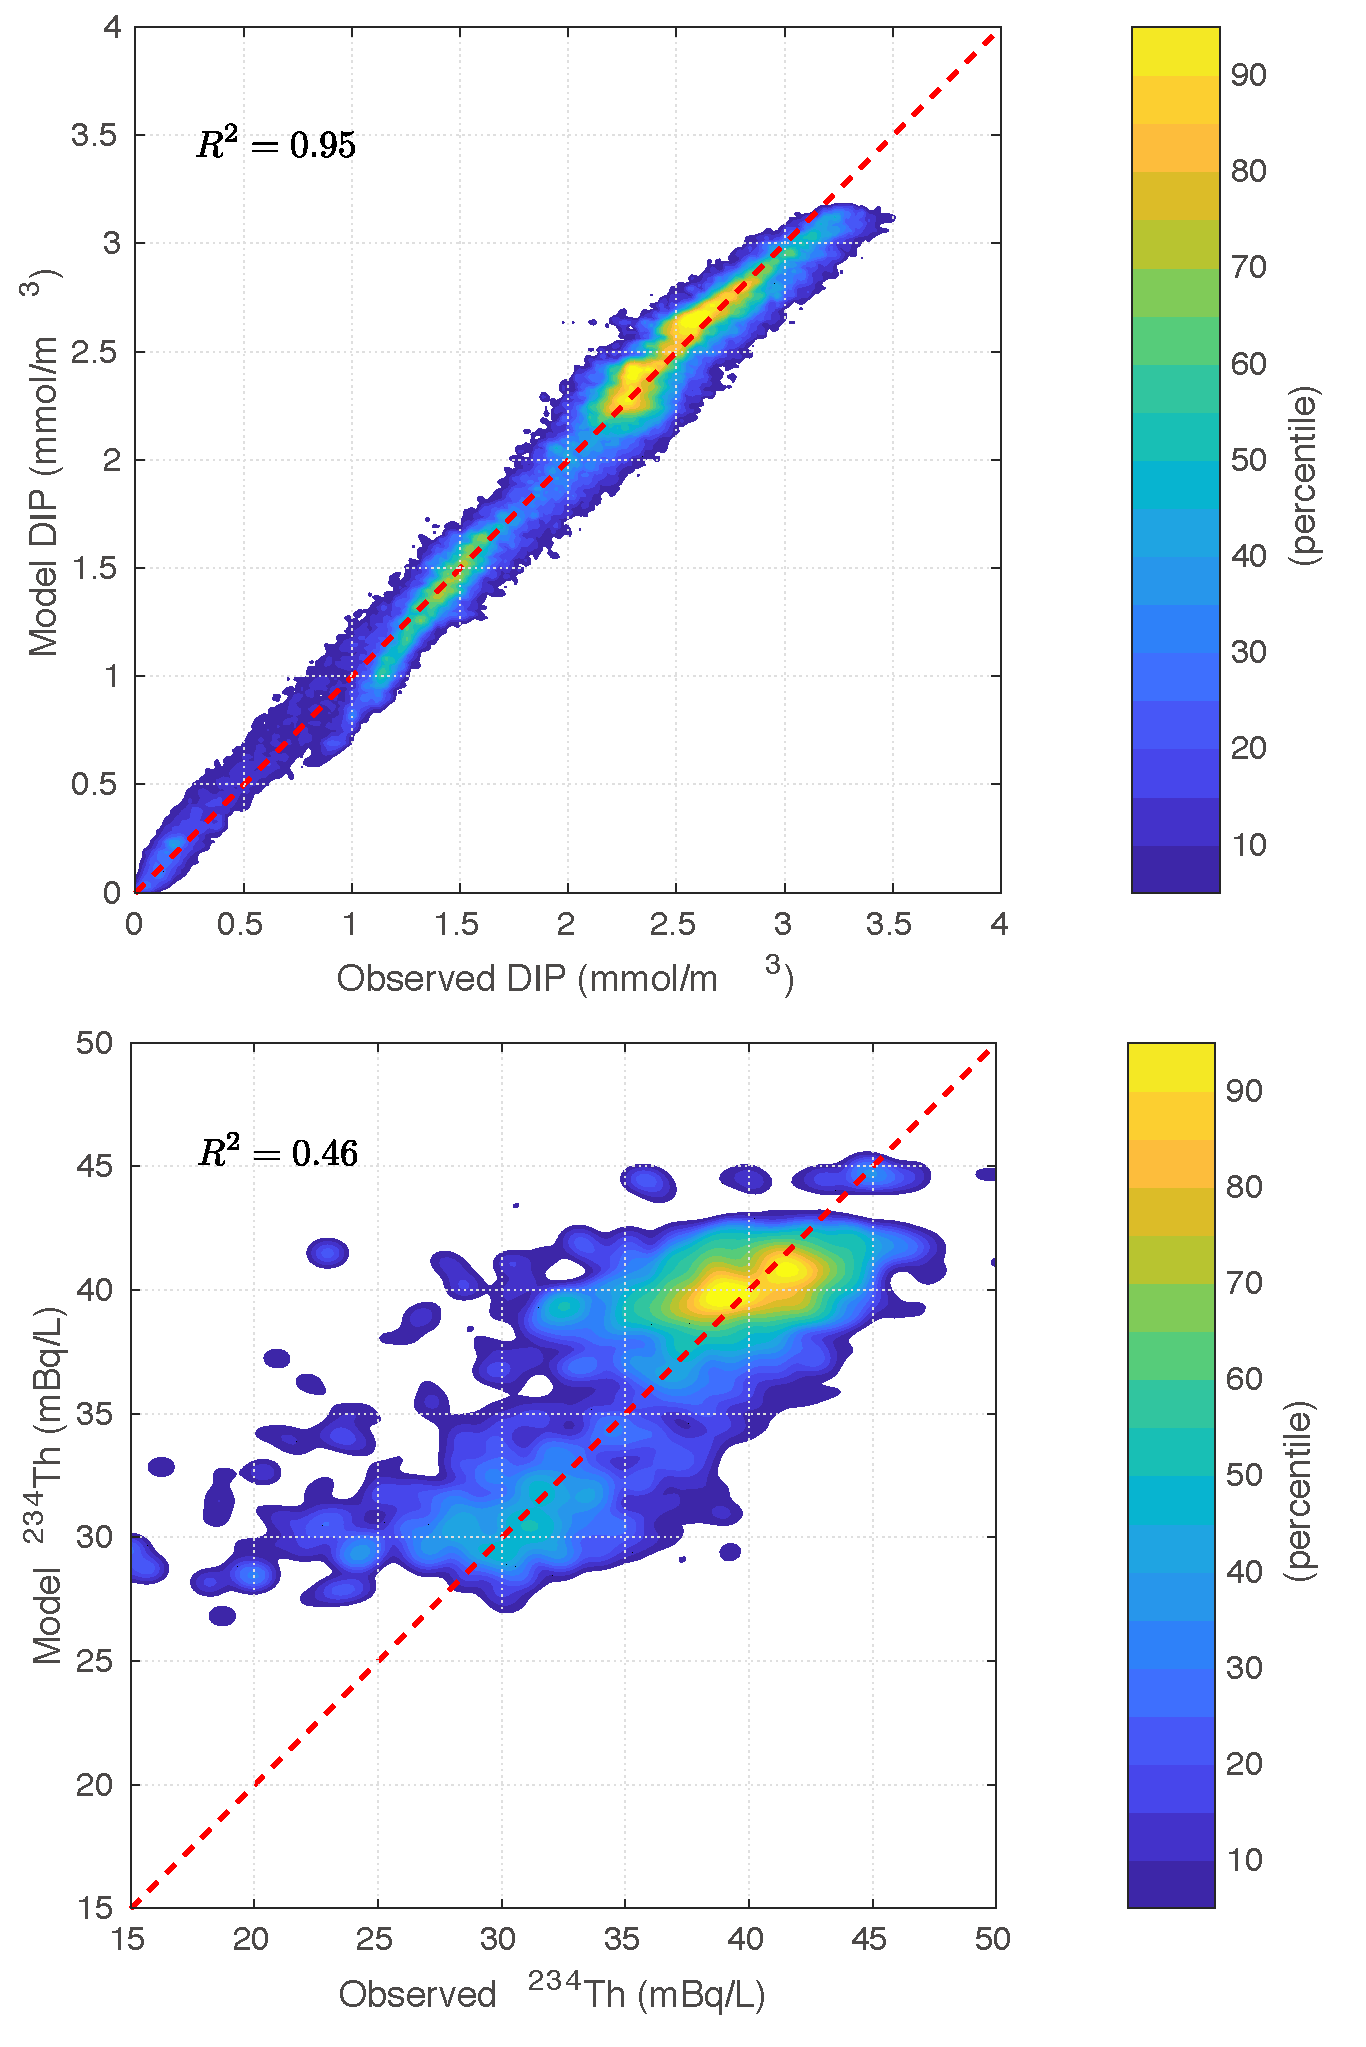
\includegraphics[width=1.0\textwidth,center]{MvsO.pdf}
\caption{Comparison of model tracers with observed ones.  1) Model DIP versus WOA2013 climatology DIP concentration. 2) Model total 234Th (dissolved + particulate) versus observation.}
\label{fig:MvsO}
\end{figure}

\clearpage
\begin{figure}[!htb]
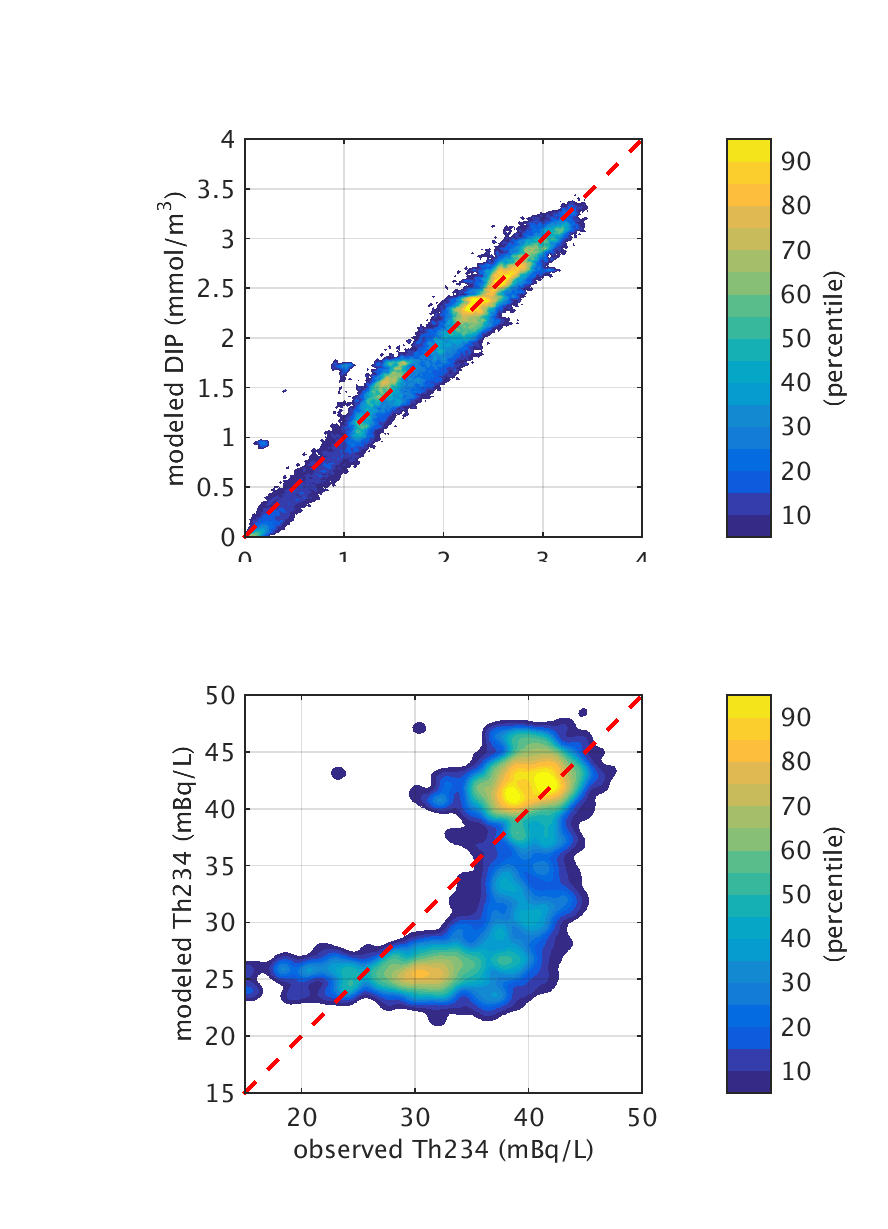
\includegraphics[width=1.0\textwidth,center]{MvsO_GB15.pdf}
\caption{Comparison of observation tracers with model based on Galbraith and Martiny \cite{Galbraith2015} C:P parameterization.  1) Model DIP versus WOA2013 climatology DIP concentration. 2) Model total 234Th (dissolved + particulate) versus observation.}
\label{fig:MvsO_GB15}
\end{figure}


\clearpage
\begin{figure}[bp!]
\includegraphics[width=1.0\textwidth,center]{hist.eps}
\caption{Histogram shows total POC, TOC, and DOC distributions based on Monte Carlo simulation. In the test, we randomly select parameter combinations ($\theta_i \sim N(\hat{\theta},\Sigma)$), with which we recalculated POC, TOC, and DOC export flux. The model was run 1000 times.}
\label{fig:mc}
\end{figure}

\clearpage
\begin{figure}[bp!]
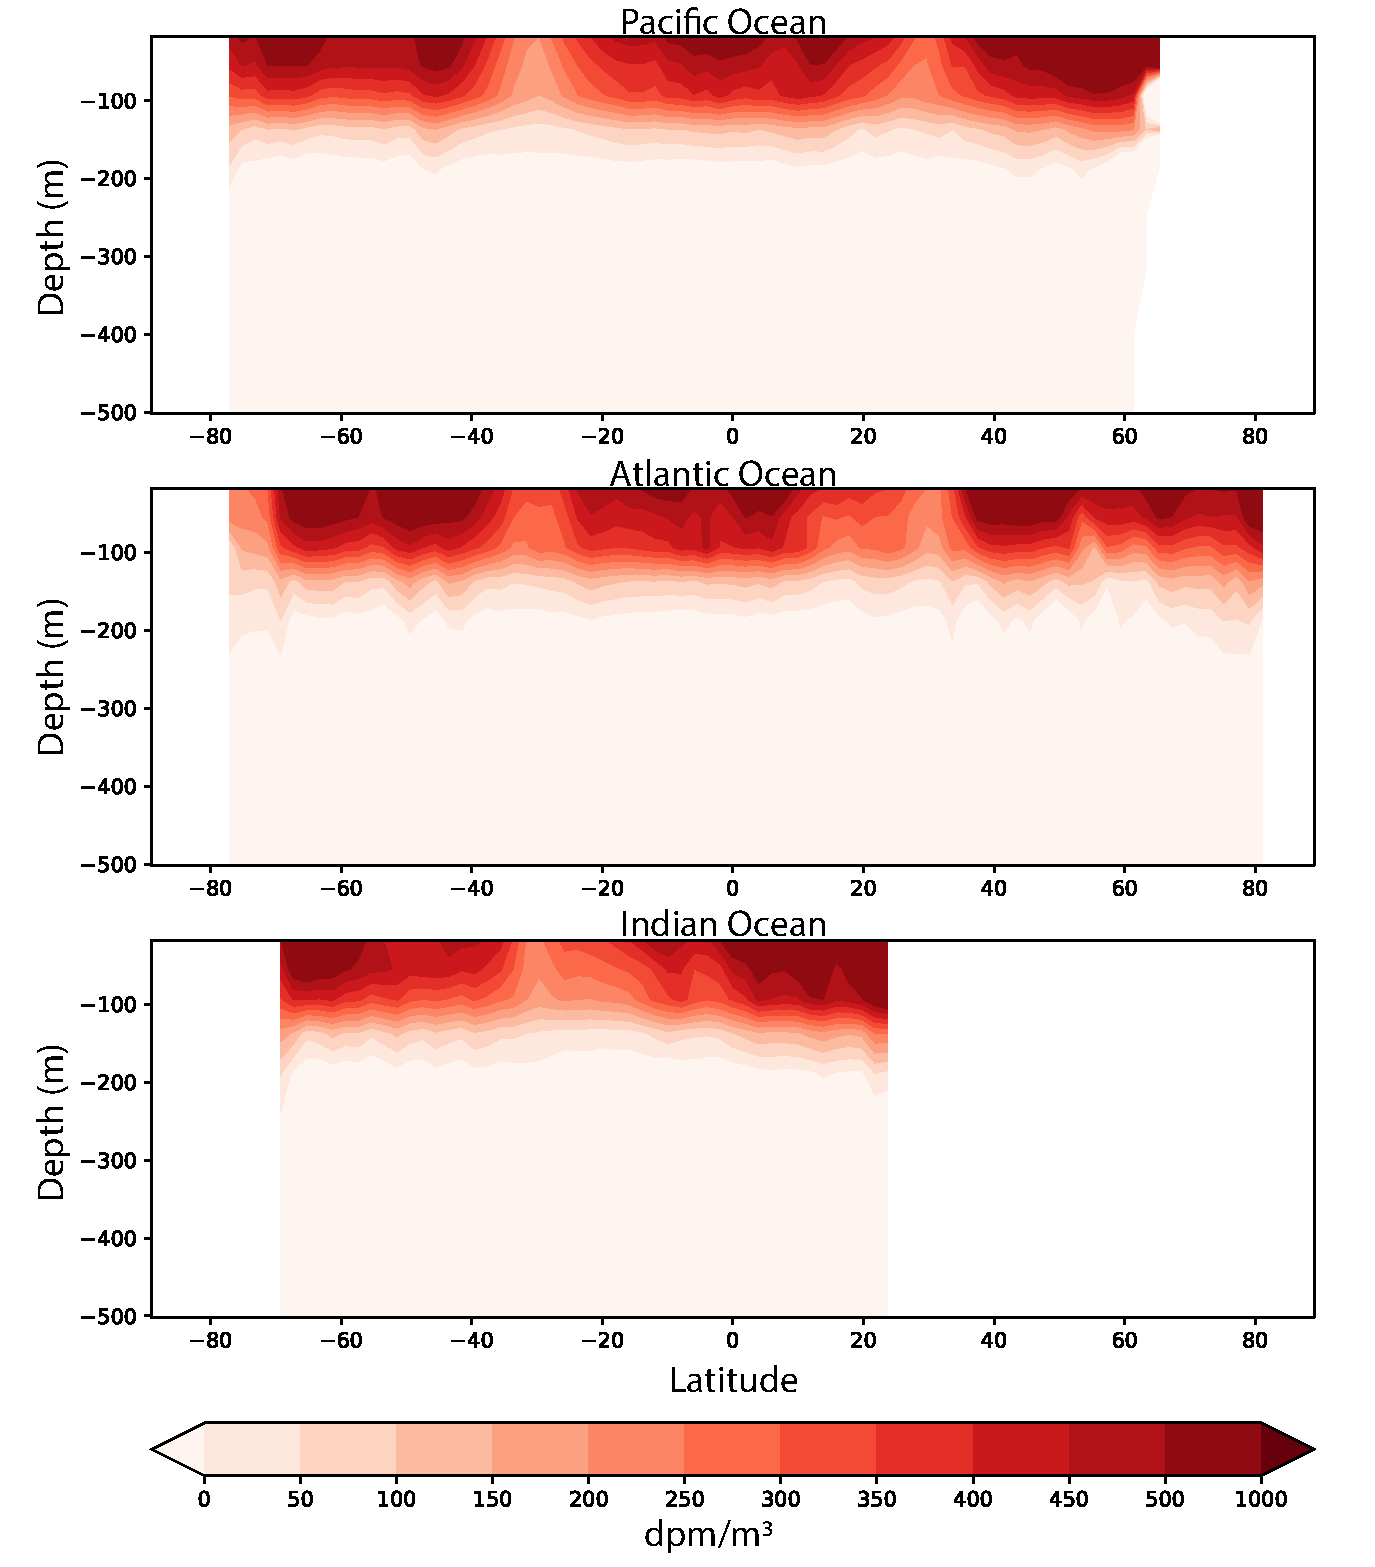
\includegraphics[width=1.0\textwidth,center]{Meridian_distribution.pdf}
\caption{Zonally mean difference between $^{238}$U and $^{234}$Th for the three major basins.}
\label{fig:Meridian_distribution}
\end{figure}

%%%%%%%%%%%%%%%%%%%%%%%%%%%%%%%%
%% Optional Appendix goes here
%
% \appendix resets counters and redefines section heads
% but doesn't print anything.
% After typing \appendix
%
%\section{Here Is Appendix Title}
% will show
% A: Here Is Appendix Title
%
% \appendix
% \section{Here is a sample appendix}
% This is an Appendix section.

% \subsection{subsection}
% This is an Appendix subsection.

% \subsubsection{subsubsection}
% This is an Appendix subsubsection.
% \begin{linenomath*}
% \begin{equation}asdf\end{equation}
% \end{linenomath*}

%%%%%%%%%%%%%%%%%%%%%%%%%%%%%%%%%%%%%%%%%%%%%%%%%%%%%%%%%%%%%%%%
%
% Optional Glossary, Notation or Acronym section goes here:
%
%%%%%%%%%%%%%%
% Glossary is only allowed in Reviews of Geophysics
% \begin{glossary}
% \term{Term}
%  Term Definition here
% \term{Term}
%  Term Definition here
% \term{Term}
%  Term Definition here
% \end{glossary}

%
%%%%%%%%%%%%%%
% Acronyms
 % \begin{acronyms}
 % \acro{Acronym}
 % Definition here
 % \acro{EMOS}
 % Ensemble model output statistics
 % \acro{ECMWF}
 % Centre for Medium-Range Weather Forecasts
 % \end{acronyms}

%
%%%%%%%%%%%%%%
% Notation
%  \begin{notation}
%  \notation{$a+b$} Notation Definition here
%  \notation{$e=mc^2$}
%  Equation in German-born physicist Albert Einstein's theory of special
% relativity that showed that the increased relativistic mass ($m$) of a
% body comes from the energy of motion of the body—that is, its kinetic
% energy ($E$)—divided by the speed of light squared ($c^2$).
%  \end{notation}

%%%%%%%%%%%%%%%%%%%%%%%%%%%%%%%%%%%%%%%%%%%%%%%%%%%%%%%%%%%%%%%%
%
%  ACKNOWLEDGMENTS



%%  REFERENCE LIST AND TEXT CITATIONS
%
% Either type in your references using
%


%
% Or, to use BibTeX:
%
% Follow these steps
%
% 1. Type in \bibliography{<name of your .bib file>}
%    Run LaTeX on your LaTeX file.
%
% 2. Run BiBTeX on your LaTeX file.
%
% 3. Open the new .bbl file containing the reference list and
%   copy all the contents into your LaTeX file here.
%
% 4. Run LaTeX on your new file which will produce the citations.
%
% AGU does not want a .bib or a .bbl file. Please copy in the contents of your .bbl file here.

% \bibliographystyle{agu08.bst}

% \begin{thebibliography}{}
% \bibliography{Thorium.bib}

\clearpage
\bibliography{Thorium}
% \clearpage
% \begin{thebibliography}{57}
% \providecommand{\natexlab}[1]{#1}
% \expandafter\ifx\csname urlstyle\endcsname\relax
%   \providecommand{\doi}[1]{doi:\discretionary{}{}{}#1}\else
%   \providecommand{\doi}{doi:\discretionary{}{}{}\begingroup
%   \urlstyle{rm}\Url}\fi

% \end{thebibliography}


\end{document}

